% Task 1.2 -- Đặc tả yêu cầu phần mềm (SRS rút gọn)
% File chỉ chứa nội dung theo quy ước; trang bìa, header/footer nằm ở report.tex (ngoài repo).

\subsection{Task 1.2 -- Đặc tả yêu cầu phần mềm}

Tài liệu này đặc tả các yêu cầu chức năng (FR) và phi chức năng (NFR) cho hệ thống đặt đồ uống không dùng tiền mặt \textbf{BrewLite}.
Mức độ ưu tiên được phân loại theo phương pháp \textbf{MoSCoW} (\emph{Must have, Should have, Could have, Won't have}).
Mọi yêu cầu đều bám sát bối cảnh, stakeholder và phạm vi đã thống nhất tại Task~1.1, đi kèm tiêu chí chấp nhận có thể kiểm chứng được (Acceptance Criteria), làm cơ sở trực tiếp cho việc mô hình hóa, thiết kế kiến trúc và viết kiểm thử tự động ở các Sprint sau.

% -------------------------------------------------------------------------
\subsubsection{Yêu cầu chức năng (Functional Requirements)}

\begin{longtable}{@{}p{1.2cm}p{2.6cm}p{4.2cm}p{1.4cm}p{6.6cm}@{}}
\toprule
\textbf{Mã} & \textbf{Tên yêu cầu} & \textbf{Mô tả} & \textbf{Ưu tiên} & \textbf{Tiêu chí chấp nhận (Acceptance Criteria)} \\
\midrule
\endhead

FR-01 & Xem danh mục đồ uống (Menu)
  & Hiển thị danh sách sản phẩm gồm hình ảnh, tên, giá cơ sở và số ly còn bán được tính từ tồn kho nguyên liệu.
  & Must
  & \begin{itemize}[leftmargin=*]
      \item Gọi \texttt{GET /products} trả về HTTP 200 kèm danh sách sản phẩm.
      \item Giao diện có đầy đủ trạng thái: \emph{loading} (skeleton), \emph{empty} (khi danh mục rỗng), \emph{error} (báo lỗi kèm nút Thử lại); thiết kế mobile-first.
      \item Món có số ly còn lại $= 0$ hiển thị nhãn ``Hết hàng'', nút chọn bị vô hiệu hóa.
    \end{itemize} \\
\addlinespace

FR-02 & Chi tiết sản phẩm \& tùy chọn
  & Xem thông tin chi tiết từng món; cho phép chọn kích cỡ (S/M/L) và topping (Kem béo, Trân châu); tự động cập nhật giá và số ly còn bán.
  & Must
  & \begin{itemize}[leftmargin=*]
      \item Gọi \texttt{GET /products/:id} trả về HTTP 200 với ID hợp lệ; trả về HTTP 404 nếu ID không tồn tại.
      \item Phụ phí chuẩn: size S (+0đ), size M (+5.000đ), size L (+10.000đ); mỗi topping (+5.000đ).
      \item Hiển thị số ly còn bán được tính theo nguyên liệu còn lại ứng với đúng tùy chọn đang chọn.
      \item Tự động vô hiệu hóa tùy chọn size hoặc topping nếu nguyên liệu tương ứng trong kho không còn đủ.
    \end{itemize} \\
\addlinespace

FR-03 & Quản lý giỏ hàng (Cart)
  & Thêm món, sửa số lượng, xóa từng món, xóa toàn bộ giỏ; tự tính tổng tiền; badge số lượng; lưu trữ qua \texttt{localStorage}.
  & Must
  & \begin{itemize}[leftmargin=*]
      \item Món cùng sản phẩm và cùng tùy chọn (size, topping) được gộp dòng và cộng dồn số lượng; khác tùy chọn tạo dòng riêng.
      \item Tổng tiền giỏ hàng tự động tính lại ngay lập tức khi thay đổi số lượng.
      \item Giữ nguyên trạng thái giỏ hàng khi người dùng tải lại trang (F5) qua \texttt{localStorage}.
      \item Chặn không cho tăng số lượng vượt quá số ly tối đa mà kho nguyên liệu hiện có thể đáp ứng.
      \item Giỏ hàng \textbf{không bị xóa} khi bấm tạo đơn; chỉ xóa khi đơn hàng tương ứng đã thanh toán thành công (\texttt{PAID}).
    \end{itemize} \\
\addlinespace

FR-04 & Đăng ký \& Đăng nhập (Xác thực \& Phân quyền)
  & Đăng ký tài khoản khách hàng, đăng nhập nhận JWT; hỗ trợ phân quyền người dùng (\texttt{CUSTOMER} và \texttt{ADMIN}).
  & Must
  & \begin{itemize}[leftmargin=*]
      \item Mật khẩu được băm một chiều bằng \texttt{bcrypt} với salt rounds $\ge 10$; không lưu mật khẩu thô.
      \item Đăng ký trùng email trả về HTTP 409 Conflict (``Email đã tồn tại'').
      \item Đăng nhập sai email hoặc mật khẩu trả về HTTP 401 Unauthorized.
      \item Đăng nhập thành công trả về HTTP 200 kèm JWT token có hạn sử dụng cấu hình từ \texttt{.env}.
      \item Phân quyền chặt chẽ ở backend: người dùng thường truy cập chức năng nhân viên bị từ chối với HTTP 403 Forbidden.
      \item Khách không tự đăng ký được tài khoản \texttt{ADMIN}; tài khoản nhân viên được khởi tạo sẵn từ biến môi trường.
    \end{itemize} \\
\addlinespace

FR-05 & Đặt đơn hàng (Create Order)
  & Người dùng đã đăng nhập gửi các món trong giỏ để tạo đơn hàng. Backend tự tính lại giá; giữ nguyên liệu trong 15 phút.
  & Must
  & \begin{itemize}[leftmargin=*]
      \item Chưa đăng nhập gọi API tạo đơn trả về HTTP 401; client điều hướng sang \texttt{/login?redirect=/cart}.
      \item Bắt buộc có header \texttt{Idempotency-Key}; gửi lại cùng key trong 15 phút trả đúng đơn cũ, không tạo đơn mới.
      \item Giỏ hàng rỗng (\texttt{items: []}) trả về HTTP 400 BadRequest.
      \item Backend tự tính lại đơn giá và tổng tiền từ cơ sở dữ liệu, không tin giá từ client.
      \item Tạo đơn thành công trả về HTTP 201 Created kèm \texttt{orderId}, \texttt{total}, \texttt{status = PENDING}, thời hạn thanh toán (15 phút); giỏ hàng được giữ nguyên.
    \end{itemize} \\
\addlinespace

FR-06 & Tồn kho theo nguyên liệu \& công thức
  & Mỗi món có định lượng nguyên liệu thô theo size và topping. Giữ nguyên liệu khi tạo đơn; hoàn lại khi đơn bị hủy hoặc quá hạn.
  & Must
  & \begin{itemize}[leftmargin=*]
      \item Định lượng: size M tốn $\times 1{,}25$, size L tốn $\times 1{,}5$ nguyên liệu so với size S; mỗi topping trừ nguyên liệu riêng.
      \item Giữ/trừ nguyên liệu ngay khi tạo đơn (\texttt{POST /orders}) trong transaction với \emph{optimistic locking}.
      \item Nếu thiếu bất kỳ nguyên liệu nào: từ chối tạo đơn với HTTP 400 (``Không đủ nguyên liệu''), giỏ hàng giữ nguyên; đảm bảo không bán vượt khi nhiều khách đặt cùng lúc.
      \item Đơn bị hủy hoặc hết hạn thanh toán (\texttt{CANCELLED}): hệ thống tự động hoàn trả đầy đủ nguyên liệu về kho đúng một lần.
      \item Khi thanh toán thành công (\texttt{PAID}) hoặc thất bại (\texttt{PAYMENT\_FAILED}): \textbf{không trừ/hoàn thêm} nguyên liệu.
    \end{itemize} \\
\addlinespace

FR-07 & Thanh toán qua Ngân hàng giả lập \& Thẻ
  & Khách thanh toán qua Ngân hàng giả lập (quét QR) hoặc quẹt thẻ tại quầy; tiền ghi nhận vào sao kê của quán.
  & Must
  & \begin{itemize}[leftmargin=*]
      \item \texttt{POST /payments} nhận \texttt{orderId}, \texttt{method: 'WALLET' | 'CARD'}, bắt buộc có \texttt{Idempotency-Key}.
      \item Chỉ cho phép thanh toán đơn của chính mình; đơn phải ở \texttt{PENDING} hoặc \texttt{PAYMENT\_FAILED} (thử lại). Số tiền lấy từ đơn hàng do backend tính.
      \item \textbf{Ngân hàng giả lập}: quét mã QR mở trang chuyển tiền (không cần đăng nhập trên điện thoại), số tiền cố định, nội dung là mã đơn; bấm ``Chuyển tiền'' ghi nhận tiền vào sao kê quán, phiên chuyển \texttt{TRANSFER\_RECEIVED}, đơn vẫn \texttt{PENDING}.
      \item \textbf{Thẻ tại quầy}: quẹt thẻ ngoài hệ thống; khi nhân viên xác nhận thì khoản tiền được ghi nhận vào sao kê.
      \item Gửi lại cùng \texttt{Idempotency-Key} trả đúng phiên cũ, không tạo phiên thanh toán mới.
    \end{itemize} \\
\addlinespace

FR-08 & Đối chiếu sao kê \& Xác nhận thanh toán (Nhân viên)
  & Nhân viên (\texttt{ADMIN}) trên trang quản trị đối chiếu sao kê để xác nhận hoặc từ chối thanh toán; hệ thống tự hoàn tiền khi từ chối.
  & Must
  & \begin{itemize}[leftmargin=*]
      \item Khách hàng \textbf{không được tự xác nhận} đơn đã thanh toán (theo yêu cầu của giảng viên).
      \item Trang quản trị tab Thanh toán tự làm mới bằng polling mỗi 4 giây, có thông báo và âm báo khi có tiền về; đưa đơn có tiền về lên đầu.
      \item Nhân viên bấm ``Xác nhận'' $\rightarrow$ phiên thành \texttt{SUCCESS}, đơn thành \texttt{PAID}, client khách hàng xóa giỏ hàng.
      \item Nhân viên bấm ``Từ chối'' $\rightarrow$ phiên thành \texttt{FAILED}, đơn thành \texttt{PAYMENT\_FAILED}, hệ thống tự động hoàn tiền trên sao kê; giỏ hàng giữ nguyên để khách thử lại.
      \item Khóa dòng (locking) chống hai nhân viên cùng thao tác hoặc xử lý lặp một phiên.
    \end{itemize} \\
\addlinespace

FR-09 & Hủy đơn hàng \& Hoàn tiền
  & Quy trình hủy đơn cho khách và duyệt hủy của nhân viên; tự động hoàn trả tiền và nguyên liệu.
  & Must
  & \begin{itemize}[leftmargin=*]
      \item Đơn chưa có tiền về: khách được bấm hủy ngay $\rightarrow$ đơn thành \texttt{CANCELLED}, hoàn nguyên liệu về kho.
      \item Đơn đã có tiền về hoặc đã \texttt{PAID} (chưa pha chế): khách gửi yêu cầu hủy $\rightarrow$ nhân viên duyệt $\rightarrow$ đơn thành \texttt{CANCELLED}, tự động hoàn đúng số tiền đã nhận trên sao kê và hoàn nguyên liệu.
      \item Đơn từ \texttt{PREPARING} trở đi không được hủy; API từ chối với HTTP 400.
      \item Mọi lần hủy đơn đang có tiền đều tự hoàn đúng số đã nhận, thực hiện đúng một lần.
    \end{itemize} \\
\addlinespace

FR-10 & Máy trạng thái đơn \& Tự hủy quá hạn
  & Quản lý vòng đời đơn qua máy trạng thái nghiêm ngặt; tự hủy đơn quá hạn thanh toán sau 15 phút.
  & Must
  & \begin{itemize}[leftmargin=*]
      \item Vòng đời hợp lệ: $\texttt{PENDING} \rightarrow \texttt{PAID} \rightarrow \texttt{PREPARING} \rightarrow \texttt{READY} \rightarrow \texttt{COMPLETED}$.
      \item Nhánh lỗi \& thử lại: $\texttt{PENDING} \rightarrow \texttt{PAYMENT\_FAILED} \rightarrow$ (khách thử lại) $\texttt{PENDING} \rightarrow \texttt{PAID}$. Tuyệt đối không chuyển thẳng $\texttt{PAYMENT\_FAILED} \rightarrow \texttt{PAID}$.
      \item Nhánh hủy: $\texttt{PENDING} \rightarrow \texttt{CANCELLED}$ hoặc $\texttt{PAID} \rightarrow \texttt{CANCELLED}$ (qua duyệt hủy).
      \item Tự động hủy đơn sau 15 phút không thanh toán: chuyển \texttt{CANCELLED} và hoàn nguyên liệu; \textbf{không tự hủy} đơn đã có tiền về (\texttt{TRANSFER\_RECEIVED}).
      \item Mọi chuyển trạng thái sai quy tắc đều bị chặn bởi \texttt{assertTransition} và trả về HTTP 400.
    \end{itemize} \\
\addlinespace

FR-11 & Bảng pha chế Barista
  & Màn hình cho nhân viên/Barista tiếp nhận đơn đã \texttt{PAID} và cập nhật tiến trình pha chế đồ uống.
  & Must
  & \begin{itemize}[leftmargin=*]
      \item Bảng pha chế hiển thị danh sách đơn đã \texttt{PAID} với đầy đủ thông tin món, kích cỡ, topping.
      \item Nhân viên cập nhật trạng thái: $\texttt{PAID} \rightarrow \texttt{PREPARING} \rightarrow \texttt{READY} \rightarrow \texttt{COMPLETED}$.
      \item Khách hàng theo dõi thấy trạng thái đơn thay đổi theo thời gian thực (báo khi đồ uống sẵn sàng).
    \end{itemize} \\
\addlinespace

FR-12 & Tra cứu lịch sử đơn \& Theo dõi đơn
  & Khách hàng xem lịch sử đơn cá nhân; nhân viên tra cứu toàn bộ đơn và sao kê cửa hàng.
  & Must
  & \begin{itemize}[leftmargin=*]
      \item Khách hàng: \texttt{GET /orders/me} chỉ xem đơn của mình; \texttt{GET /orders/:id} xem chi tiết món, giá, trạng thái và số tiền đã hoàn; xem đơn người khác bị từ chối với HTTP 403.
      \item Nhân viên: Tab Lịch sử đơn xem mọi đơn ở mọi trạng thái, lọc theo trạng thái, tìm theo mã đơn/email khách, phân trang; xem chi tiết phiên thanh toán (ai duyệt/từ chối, lý do) và sao kê tiền vào/hoàn tiền.
    \end{itemize} \\
\addlinespace

FR-13 & Khuyến mãi (Voucher) \& Điểm thưởng
  & Áp dụng mã giảm giá khi đặt đơn; tích lũy điểm thưởng khi đơn thanh toán thành công.
  & Must
  & \begin{itemize}[leftmargin=*]
      \item Mỗi đơn tối đa một mã giảm giá; mỗi tài khoản dùng mỗi mã tối đa 3 lần.
      \item Giữ lượt dùng khi tạo đơn, chốt khi \texttt{PAID}, hoàn lại lượt khi đơn bị hủy; mã sai/hết hạn báo lỗi HTTP 400.
      \item Tích điểm: mỗi 10.000đ thực trả (sau giảm giá) $= 1$ điểm (làm tròn xuống). Cộng điểm khi đơn chuyển \texttt{PAID}; thu hồi đúng số điểm đã cộng khi hủy đơn \texttt{PAID}.
    \end{itemize} \\
\addlinespace

FR-14 & Quản lý menu, giá \& nhập kho nguyên liệu (Admin mở rộng)
  & Giao diện chỉnh sửa menu, giá bán, công thức và nhập kho nguyên liệu trực tiếp trên web.
  & Won't
  & Nằm ngoài phạm vi MVP theo thỏa thuận tại Task~1.1; số liệu mẫu được nạp sẵn qua database seed, chỉnh sửa trực tiếp trong CSDL khi cần. \\
\addlinespace

FR-15 & Đổi điểm thưởng \& Tích hợp cổng thanh toán thật
  & Đổi điểm tích lũy lấy đồ uống/voucher; tích hợp cổng thanh toán ngân hàng thật (VNPay/MoMo thật); thanh toán tiền mặt.
  & Won't
  & Nằm ngoài phạm vi MVP (Out-of-scope). \\
\bottomrule
\end{longtable}

% -------------------------------------------------------------------------
\subsubsection{Yêu cầu phi chức năng (Non-Functional Requirements)}

\begin{longtable}{@{}p{1.4cm}p{3.2cm}p{5.0cm}p{1.4cm}p{5.0cm}@{}}
\toprule
\textbf{Mã} & \textbf{Nhóm yêu cầu} & \textbf{Mô tả} & \textbf{Ưu tiên} & \textbf{Tiêu chí chấp nhận} \\
\midrule
\endhead

NFR-01 & Hiệu năng (Performance)
  & Tốc độ xử lý yêu cầu và khả năng đáp ứng đồng thời trong giờ cao điểm.
  & Must
  & \begin{itemize}[leftmargin=*]
      \item Thời gian phản hồi API (GET/POST với dữ liệu mẫu) dưới 500ms.
      \item Hệ thống đáp ứng đồng thời tối thiểu 50 người dùng mà không xảy ra lỗi sập dịch vụ.
    \end{itemize} \\
\addlinespace

NFR-02 & Bảo mật (Security)
  & Bảo vệ thông tin người dùng, tính toàn vẹn của giao dịch và phân quyền nghiêm ngặt.
  & Must
  & \begin{itemize}[leftmargin=*]
      \item Mật khẩu băm một chiều với \texttt{bcrypt} ($\text{salt rounds} \ge 10$).
      \item Xác thực và phân quyền qua JWT; secret không xuất hiện trên repository hay log CI.
      \item Phân quyền chặt chẽ \texttt{CUSTOMER}/\texttt{ADMIN} ở backend (từ chối 403 Forbidden).
      \item Áp dụng transaction và optimistic locking để chống trừ nguyên liệu/tiền hai lần.
    \end{itemize} \\
\addlinespace

NFR-03 & Tính khả dụng (Usability \& PWA)
  & Trải nghiệm người dùng thân thiện, tối ưu cho thiết bị di động.
  & Must
  & \begin{itemize}[leftmargin=*]
      \item Thiết kế theo chuẩn mobile-first; tương thích tốt trên màn hình từ 360px trở lên.
      \item Đầy đủ trạng thái giao diện: loading, empty, error.
      \item Hỗ trợ cài đặt PWA lên màn hình chính điện thoại, mở ở chế độ standalone.
    \end{itemize} \\
\addlinespace

NFR-04 & Khả năng triển khai (DevOps)
  & Đóng gói chuẩn hóa và tự động hóa quy trình phân phối sản phẩm.
  & Must
  & \begin{itemize}[leftmargin=*]
      \item Đóng gói ứng dụng bằng Docker; có \texttt{docker-compose.yml} chạy được frontend, backend và PostgreSQL ở local.
      \item Pipeline CI/CD tự động chạy kiểm tra chất lượng (Lint $\rightarrow$ Test $\rightarrow$ Build) trước khi merge PR.
      \item Môi trường Production triển khai trên Cloud có chứng chỉ HTTPS/SSL hợp lệ và endpoint \texttt{GET /health} trả về HTTP 200.
    \end{itemize} \\
\bottomrule
\end{longtable}

% -------------------------------------------------------------------------
\subsubsection{Sơ đồ use-case tổng quát}

Hình~\ref{fig:usecase-overview} mô tả toàn bộ các ca sử dụng (use-case) của hệ thống BrewLite, làm rõ ranh giới giữa actor chính (\textbf{Khách hàng}), actor quản trị/pha chế (\textbf{Nhân viên / Barista}), dịch vụ hỗ trợ (\textbf{Ngân hàng giả lập}) và các chức năng ngoài phạm vi MVP.

\begin{figure}[htbp]
  \centering
  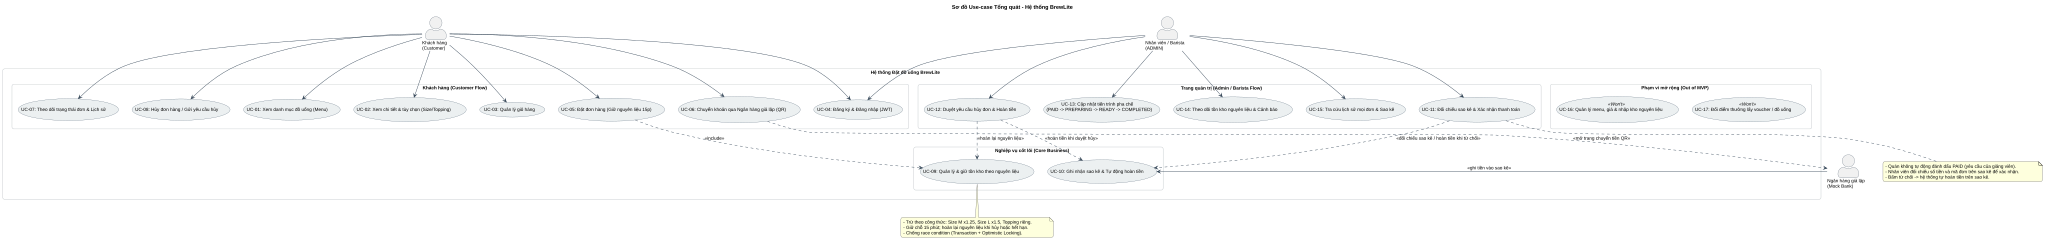
\includegraphics[width=0.98\textwidth]{docs/requirements/usecase-overview.svg}
  \caption{Sơ đồ use-case tổng quát hệ thống BrewLite}
  \label{fig:usecase-overview}
\end{figure}

Trong sơ đồ:
\begin{itemize}
  \item \textbf{Khách hàng} thực hiện luồng nghiệp vụ mua hàng: Xem menu $\rightarrow$ Xem chi tiết \& tùy chọn $\rightarrow$ Quản lý giỏ hàng $\rightarrow$ Đăng ký/Đăng nhập $\rightarrow$ Đặt đơn hàng $\rightarrow$ Chuyển khoản qua Ngân hàng giả lập $\rightarrow$ Theo dõi trạng thái đơn (hoặc Gửi yêu cầu hủy đơn).
  \item Use-case \textbf{Đặt đơn hàng} bắt buộc bao gồm (\texttt{<<include>>}) use-case \textbf{Quản lý \& giữ tồn kho theo nguyên liệu} nhằm đảm bảo tính toàn vẹn tồn kho theo công thức và chống bán vượt khi nhiều khách đặt cùng lúc.
  \item \textbf{Ngân hàng giả lập} tiếp nhận yêu cầu chuyển khoản (quét mã QR) từ khách hàng, tự động ghi nhận tiền vào \textbf{Sao kê của quán} và xử lý hoàn tiền khi đơn bị từ chối/hủy.
  \item \textbf{Nhân viên / Barista (\texttt{ADMIN})} thao tác trên trang quản trị: Đối chiếu sao kê để \emph{Xác nhận} (chuyển đơn sang \texttt{PAID}) hoặc \emph{Từ chối} thanh toán (kích hoạt tự hoàn tiền); Duyệt yêu cầu hủy đơn; Cập nhật bảng pha chế (\texttt{PAID} $\rightarrow$ \texttt{PREPARING} $\rightarrow$ \texttt{READY} $\rightarrow$ \texttt{COMPLETED}); Theo dõi tồn kho nguyên liệu và Tra cứu lịch sử đơn.
  \item Các use-case \textbf{Quản lý menu, giá, nhập kho nguyên liệu} và \textbf{Đổi điểm thưởng} được đánh dấu mức \emph{Won't} do thuộc phạm vi mở rộng sau MVP.
\end{itemize}
